% =====================================================================
% Stage 1 Concept and Feasibility Report -- WORKING DRAFT
% Project I (247-519-VA) | Andrei Prodan (6317869)
%
%  - The proposal is frozen and is NOT extended here: requirements
%    REQSU-01..08, risks R1..R3 and needs N1..N6 are exactly as submitted.
%  - Every test result is entered first as a logbook entry (Appendix A,
%    raw output in logs/L-xx_*.txt), then summarised in Sections 3-6.
%  - Anything still to be supplied by the author is marked \pend{...}.
%  - Claims C1.. and logbook entries L-02.. are new in this report.
%  - Ideas that go beyond the proposal live in notes/PRIVATE_notes.md,
%    not in this document.
% =====================================================================
% Uses the real IEEEtran class when IEEEtran.cls is present; otherwise a two-column
% article stand-in with similar margins, so the file always compiles.
\IfFileExists{IEEEtran.cls}{\documentclass[conference]{IEEEtran}}{\documentclass[10pt,twocolumn]{article}}
\makeatletter
\@ifclassloaded{IEEEtran}{}{%
  \usepackage[letterpaper,top=0.75in,bottom=1in,left=0.625in,right=0.625in,columnsep=0.25in]{geometry}
  \usepackage{mathptmx}
  \providecommand{\IEEEauthorblockN}[1]{#1\\}
  \providecommand{\IEEEauthorblockA}[1]{\small #1}
  \newenvironment{IEEEkeywords}{\par\small\noindent\textit{Index Terms}---}{\par}
}
\makeatother
\usepackage[T1]{fontenc}
\usepackage{amsmath,amssymb}
\usepackage{booktabs,tabularx,array,colortbl}
\usepackage{graphicx}
\usepackage{adjustbox}
\usepackage{verbatim}
\usepackage{tikz}
\usetikzlibrary{arrows.meta,positioning}
\usepackage{xcolor}

\emergencystretch=2em
\renewcommand{\arraystretch}{1.1}
\newcolumntype{Y}{>{\raggedright\arraybackslash}X}
\newcommand{\pend}[1]{\textsf{\textbf{[PENDING: #1]}}}
\newcommand{\req}[1]{\textsc{reqsu-}#1}
\newcommand{\sm}{\footnotesize}
\newcommand{\fitcol}[1]{\begin{adjustbox}{max width=\columnwidth}#1\end{adjustbox}}

\begin{document}
\title{Logbook Extracts and Optional Appendix\\Project I, Stage 1 Concept and Feasibility Report}
\author{\IEEEauthorblockN{Andrei Prodan (6317869)}
\IEEEauthorblockA{Companion to the Gate 1 report (main.pdf), 20 November 2026}}
\date{}
\maketitle

\appendix
\section{Logbook Extracts}
\begin{table*}[!t]
\caption{Logbook index}
\centering\footnotesize
\begin{tabularx}{\textwidth}{@{}l l Y@{}}
\toprule
Entry & Date & Content\\
\midrule
L-02 & 2026-10-23, 2026-11-06 & Research on links (ESP-NOW, Bluetooth LE, external transceiver) and positioning (trilateration, triangulation); entry below.\\
L-03 & 2026-11-13 & Session with instructor on storing connectivity between wireless agents and a beacon. The adjacency matrix is the relevant part (Section~3); sparse (CSR) storage is optional background (Appendix~B). The HTML/JS simulator \texttt{beacon\_app.html} is to be extended with the RSSI data gathered in testing. Files: \texttt{beacon\_storage.tex/pdf}, \texttt{beacon\_sim.py}, \texttt{beacon\_app.html}, \texttt{beacon\_network.png}.\\
L-04 & 2026-11-13 & Test 1a, below.\\
L-05 & 2026-11-13 & Three ESP32 boards in shipping: the beacon and two further reference points, which give the three reference points 2D trilateration needs (L-02). Received by 2026-11-15 (L-09). Tests 2--5 and the position measurements remain open.\\
L-06 & 2026-11-13 & Criteria and weights for Section~2 (coverage 0.35, uncertainty 0.25, buildability 0.25, cost 0.15), written before scoring; chosen by the assistant at the author's request; the author confirmed them on 2026-11-16.\\
L-07 & 2026-11-13 & Tests 6 and 7 on the watch screen: 24/24 and 12/12, overall PASS, touch input.\\
L-08 & 2026-11-13 & Test 10, subgroup selection on the watch: hand cases 8/8, 3$\times$1000 random trials, overall PASS.\\
L-09 & 2026-11-15 & Boards arrive; Test 1b, ESP-NOW link watch$\leftrightarrow$B0, R1, R2: 1242 of 1350 round trips (92.0\,\%) over 15 rounds; criterion missed once in the first two rounds (R1, 26), met in 39 of 45 board-rounds overall.\\
L-10 & 2026-11-16 & BLE advertising switched off on R1 only: R1 97.3\,\% against 94.0\,\% (B0) and 91.0\,\% (R2) with BLE on, in the same session and with positions swapped; BLE on the boards probably costs 5--7 points of delivery.\\
L-11 & 2026-11-16 & Test 1b repeated with BLE off on all three boards, 1--2\,m: 447 of 450 round trips (99.3\,\%), every board in every round 29 or 30; pass line RT $\ge 27$ met in 15 of 15 board-rounds. BLE advertising was the main cause of the L-09 loss.\\
L-12 & 2026-11-17 & Tests 4, 5 and 11 over ESP-NOW, BLE off: beacon B0, scripted R1 and R2, watch with touch consent, 10 runs: request reached the watch 10/10, report 10/10, size, leader and members correct 10/10, profile sent only after ACCEPT (5 sent, 3 blocked, 0 violations). Overall PASS.\\
L-13 & 2026-11-17 & 30\,m hallway variant of the range test, BLE off, boards together at one end: B0 answered 28 of 30 at 10\,m, 18 at 20\,m, and 13, 9, 8 at 30\,m. Pass line (B0 $\ge 27$ in each 30\,m round) not met. People were walking in the hallway.\\
L-14 & 2026-11-17 & Delivery against distance, same hallway, B0 beside the laptop: B0 14 and 15 of 30 at 15\,m, 13 and 15 at 25\,m; R1 and R2 21--30 at both distances. No pass line (curve).\\
L-15 & 2026-11-17 & B0 moved next to R1 and R2, away from the laptop; 30\,m $\times 3$ then 25\,m $\times 2$: B0 24, 26, 21 at 30\,m and 15, 16 at 25\,m. L-13 pass line (B0 $\ge 27$ in each 30\,m round) not met again. People in the way, so low reliability.\\
L-16 & 2026-11-18 & C6 position run in a 3\,m$\times$4\,m room: B0, R1, R2 at (0,0), (3,0), (0,4)\,m, 3 calibration rounds, 6 test spots. Mean error 1.94\,m against 1.25\,m allowed and 1.24\,m for guessing the centre. Not met. Confined to the room: 1.20\,m (chosen after the data).\\
L-17 & 2026-11-20 & Graph simulation of the system (10 participants plus the beacon, 2000 trials per range, seed 20261120): node degree, connectivity, detached groups, old-group matrix, connectivity-based leader. Simulated only. Code \texttt{code/graph\_sim.py}, output \texttt{logs/L-17\_graph\_sim.txt}, demonstrator \texttt{code/beacon\_app\_v2.html}.\\
L-18 & 2026-11-20 & Group-formation model in \texttt{beacon\_app\_v3.html}: 0/1 links, free random walk, coordinator and temporary beacon (local to whole arena), request relayed hop by hop along links, consent chance, group size limited or not, leader with most outside links locked at formation, release. 20 seeds $\times$ 300\,s per setting. Simulated only. Output \texttt{logs/L-18\_group\_model\_sim.txt}.\\
L-19 & 2026-11-20 & Graph neural network, worked by hand on three nodes, and the planned Stage 2 uses (relaying toward skilled nodes, leader quality, acceptance and group success). Calculated by hand, checked in code; nothing trained. Figures \texttt{figures/fig\_graph\_example\_bw.png}, \texttt{fig\_layers\_bw.png}.\\
\bottomrule
\end{tabularx}

\end{table*}
L-01 (early brainstorming) predates the proposal and is not reproduced here.

\subsection*{L-02, 2026-10-23 and 2026-11-06, assumed: link and positioning research}
\textbf{Objective.} Compare candidate links and positioning methods for R1 and R2. \textbf{Class.} Secondary sources only, nothing measured, so every figure is \emph{assumed}. Only the ESP-NOW description cites a source (Espressif, \texttt{espressif.com/en/solutions/\allowbreak low-power-solutions/\allowbreak esp-now}); the range figures came from an AI assistant (Gemini) and were not checked against a primary source, so they stay \emph{assumed} until measured (C3).

\begin{center}\footnotesize\setlength{\tabcolsep}{4pt}
\fitcol{\begin{tabular}{@{}l l l p{2.6in}@{}}
\toprule
Link & Clear / outdoors & Obstacles / indoors & Notes\\
\midrule
Wi-Fi 2.4\,GHz (ESP32-S3) & 35--50\,m & 15--20\,m & ESP-NOW runs on this radio\\
Bluetooth 5.0 & 30--40\,m & 10--15\,m & standard mode\\
BLE Long Range (Coded PHY) & 100--200+\,m & 20--40\,m & \\
nRF24L01 (2.4\,GHz) & 30--100\,m & 10--30\,m & hurt by walls, concrete floors, 2.4\,GHz traffic; external antenna: 700--1000\,m outdoors, 30--100+\,m indoors; external modules needed\\
\bottomrule
\end{tabular}}
\end{center}

\textbf{Positioning notes.} Trilateration: distances from three or more reference points; in 2D three circles give one position (one point gives a circle, two give two intersections). In 3D three points leave two positions and four are used in the real world, the fourth correcting a clock error as in GPS, which is not needed here. Triangulation: two or more angular lines of sight; in 2D a baseline between two points and two measured angles; needs direct line of sight. RSSI: reference points 5--10\,m apart, works with any ESP32 module, precision not required. Wi-Fi FTM/RTT: ESP32-S and -C series only. \textbf{To look into:} multipath interference and signal attenuation (indoor transmission).

\textbf{Reasons recorded} (author to confirm wording).
\begin{itemize}\setlength\itemsep{0pt}
\item ESP-NOW stays a candidate: built into the watch's chip, fast and low power, suits one beacon controlling many watches, and the beacon only needs an ESP-family board.
\item External transceiver not preferred: needs external modules at both ends (cost), the watch has only Wi-Fi and BLE (proposal), and indoor range is hurt by walls and 2.4\,GHz traffic.
\item Triangulation set aside: needs angle measurements and direct line of sight, while RSSI from received packets gives strength, not direction.
\item Wi-Fi FTM/RTT set aside: only on ESP32-S and -C series; RSSI works on any ESP32 module and the application does not need precise ranging.
\item Undecided: ESP-NOW or BLE as the link; the author leans to BLE Long Range for its 20--40\,m through obstacles but is not sure.
\end{itemize}

\subsection*{L-04, 2026-11-13, measured: Test 1a, can the watch run the candidate links?}
{\sloppy\textbf{Objective.} Check that ESP-NOW and BLE initialise and run together on the watch (supports \req{04}, R1). \textbf{Device.} Waveshare ESP32-S3-Touch-AMOLED-2.06, Arduino IDE, Arduino-ESP32 core 3.3.12, IDF v5.5.5, chip ESP32-S3 rev 2, 240\,MHz, flash 33{,}554{,}432\,B (32\,MiB), PSRAM 8\,MiB. \textbf{Code.} \texttt{code/test1a\_watch\_link\_check.ino}. \textbf{Pass criterion} (stated in the sketch header before the run): steps 1--7 pass and no send failures in a 30\,s soak. \textbf{Environment and power:} indoors, USB-powered; antenna orientation not recorded. \textbf{N:} one run, 31 broadcasts. \textbf{Result:} OVERALL PASS; tx OK 31, tx fail 0, received from others 0.}

\textbf{Anomalies and limits.} Step 7 reports pass unconditionally after the advertising call, so it alone does not show BLE visibility. ESP-NOW callback success is not proof of reception. The sketch's setup note said 16\,MB flash; the board reports 32\,MiB, which does not affect the result.

\textbf{Addendum, 2026-11-13, measured (BLE only).} Using Microsoft Bluetooth LE Explorer on a PC, the author found the watch's advertisement (name \texttt{T1a-watch}) and paired with it. Not recorded: PC: Lenovo ThinkPad Yoga 11e, Windows 10; the PC was close to the watch and the first attempt succeeded. This shows another device can discover and pair over BLE; it does not show message delivery, range, ESP-NOW reception, or reception by the beacon.

\textbf{Raw serial output} (\texttt{logs/L-04\_test1a\_serial.txt}):
{\fontsize{5.5}{6.5}\selectfont\verbatiminput{logs/L-04_test1a_serial.txt}}

\subsection*{L-07, 2026-11-13, planned: Tests 6 and 7, filtering and consent gate on the watch}
\textbf{Objective.} Check that the watch filters requests correctly (\req{01}, R3) and shares profile data only after the participant accepts on the watch (\req{06}). \textbf{Code.} \texttt{code/test6\_7\_filter\_consent.ino}. \textbf{Model.} Eight abstract skills A--H as a bitmask; a request is relevant if the participant is available and shares at least one skill. \textbf{Test 6.} 24 hand-written cases (skill rule alone, availability alone, combined); pass: 24 of 24. \textbf{Test 7.} 12 runs (4 accept, 3 reject, 3 timeout, 2 non-matching) on the watch screen; pass: every run as expected, profile sent exactly once in each accept run and never otherwise, zero violations. \textbf{Limits.} The tap stands in for the final interface and the TX line for the radio send, so \req{06} is supported on the watch side only. \textbf{Input mode:} touch screen (touch controller found at 0x38). \textbf{Result, same day:} Test 6, 24 of 24 correct. Test 7, 12 of 12 runs as expected: runs 1--4 accepted, 5--7 rejected, 8--10 timed out, 11--12 filtered; profile sent 4 times (accept runs only), 6 requests blocked by the gate, 0 violations. Overall PASS, first attempt. Serial log: \texttt{logs/L-07\_test6\_7\_serial.txt}. The sketch first failed to compile (enum types used before definition by the IDE's auto-prototypes) and was fixed before this run. \textbf{Limits.} Abstract skills, tap in place of the final interface, TX line in place of the radio; the 12 runs are scripted, so this shows the logic is correct, not that people respond reliably.

\subsection*{L-08, 2026-11-13: Test 10, subgroup selection covers the task skills}
\textbf{Objective.} Check that a selection rule picks a subgroup covering every required skill whenever one exists, and says so honestly when none does (\req{08}, C5). \textbf{Code.} \texttt{code/test10\_selection.ino}. \textbf{Model.} Eight abstract skills A--H as a bitmask; rule under test: greedy cover (repeatedly pick the available participant adding the most missing required skills). A candidate rule, not fixed by the proposal. \textbf{Part A.} 8 hand-worked cases; pass 8 of 8. \textbf{Part B.} 3 batches of 1000 random trials (seeds 1--3; rosters of 2--10; each skill held with probability 1/4; 80\,\% available; task needs 2--4 skills), checked by two independent methods (coverage test, brute-force minimum subgroup). Pass, in every batch: $\ge 90\,\%$ of feasible trials covered, 0 invalid picks, 0 false ``covered'' claims, at least 100 feasible and 1 infeasible trial; subgroup size reported only. \textbf{Result.} Part A 8/8. Feasible trials 440, 418, 444 (infeasible 560, 582, 556): 100.0\,\% covered in each, 0 invalid picks, 0 false claims. Mean size greedy 1.83 against minimum 1.82; equal to the minimum in 99.4\,\% of covered trials, worst excess one participant (hand case 3 shows a non-minimal pick on purpose). Overall PASS, first run; run time 127\,ms. The watch's figures matched my host check exactly, as expected from fixed seeds. Result summary: \texttt{logs/L-08\_test10\_summary.txt}. \textbf{Limits.} This rule covers the task whenever a valid subgroup exists, so the 90\,\% threshold is met by construction; the informative results are the zero false claims and the size. Abstract skills, simulated rosters, no radio: reaching the chosen participants is R1 and R2.

\subsection*{L-09, 2026-11-15: boards arrive; Test 1b, ESP-NOW link between the watch and the three boards}
\textbf{Objective.} Check that the three boards start both radio stacks and exchange ESP-NOW frames with the watch (C2, \req{04}). \textbf{Hardware.} Three ELEGOO ESP32 boards (ESP32-D0WD-V3 rev 3.1, dual core, 240\,MHz), labelled B0 (beacon, MAC 68:09:47:5F:C6:F4), R1 (68:09:47:5F:BE:38) and R2 (68:09:47:5F:A7:AC). \textbf{Code.} \texttt{code/node\_link\_board.ino} on the boards, \texttt{code/node\_link\_watch.ino} on the watch. \textbf{Method.} The watch sends 30 numbered ESP-NOW pings, 100\,ms apart; each board answers every ping it hears with a reply carrying its count of pings heard and the signal strength (RSSI) it measured. The watch counts replies (RT, of 30). Indoors, one watch on a desk edge, boards on a bed; each board about 1\,m from the watch. \textbf{Pass (set before running).} All six start-up steps pass on each board, and $\mathrm{RT}\ge 27$ of 30 for each board in both of the first two rounds. \textbf{Board start-up.} 6 of 6 steps PASS on B0, R1 and R2 (Wi-Fi station mode, ESP-NOW init, callbacks, broadcast peer, BLE init, BLE advertising); heap free 215{,}712\,B at boot and 77{,}688\,B after both stacks. R1's first upload failed with a serial error and succeeded after lowering the upload speed.

\textbf{Arrangements.} Rounds 1--5: boards in a row on the bed on their original cables (R2 on a wall charger through a meter cable, R1 on a braided cable, B0 on a thin cable to the laptop, beside the laptop). Rounds 6--15 ($^{*}$, exploratory, after the first two rounds missed the criterion): the author first swapped the R1 and R2 cables without moving the boards, then moved the boards with the original cables, then rotated the boards around the three cable positions, repeating some positions to see whether results recurred. The round number of each arrangement was not recorded, so no per-arrangement conclusion is drawn. Values for rounds 2--15 were read from the watch's history screen and agree with the photographs of the individual rounds; round 12 comes from the history screen only.

\begin{center}\footnotesize\setlength{\tabcolsep}{4pt}
\fitcol{\begin{tabular}{@{}c ccc c ccc@{}}
\toprule
Round & \multicolumn{3}{c}{RT of 30} & & \multicolumn{3}{c}{RSSI at watch (dBm)}\\
 & B0 & R1 & R2 & & B0 & R1 & R2\\
\midrule
1 & 27 & 28 & 28 & & $-61$ & $-71$ & $-64$\\
2 & 27 & \textbf{26} & 27 & & $-61$ & $-78$ & $-67$\\
3 & 28 & 28 & 30 & & $-60$ & $-74$ & $-64$\\
4 & 29 & \textbf{25} & 27 & & $-58$ & $-71$ & $-64$\\
5 & 28 & 28 & 27 & & $-69$ & $-71$ & $-67$\\
6$^{*}$ & 28 & \textbf{25} & 28 & & $-64$ & $-66$ & $-63$\\
7$^{*}$ & 28 & 27 & 29 & & $-59$ & $-59$ & $-63$\\
8$^{*}$ & 29 & \textbf{25} & 28 & & $-60$ & $-61$ & $-59$\\
9$^{*}$ & \textbf{26} & 27 & 27 & & $-61$ & $-62$ & $-61$\\
10$^{*}$ & 28 & 27 & 29 & & $-62$ & $-61$ & $-59$\\
11$^{*}$ & 27 & 27 & 27 & & $-60$ & $-64$ & $-62$\\
12$^{*}$ & 28 & 29 & 28 & & $-61$ & $-63$ & $-59$\\
13$^{*}$ & 29 & 27 & 27 & & $-61$ & $-65$ & $-59$\\
14$^{*}$ & \textbf{26} & 30 & 28 & & $-63$ & $-64$ & $-59$\\
15$^{*}$ & 28 & 29 & 28 & & $-63$ & $-64$ & $-60$\\
\midrule
Total of 450 & 416 & 408 & 418 & & & & \\
Rate & 92.4\,\% & 90.7\,\% & 92.9\,\% & & & & \\
\bottomrule
\end{tabular}}
\end{center}
\textbf{Result.} 1242 of 1350 pings answered (92.0\,\%). The criterion was \emph{not fully met}: in round 2, R1 gave 26 (B0 and R2 gave 27). Over all 15 rounds, $\mathrm{RT}\ge 27$ held in 39 of 45 board-rounds (R1 below 27 in rounds 2, 4, 6 and 8; B0 in rounds 9 and 14; R2 never), and all three boards reached 27 together in 9 of 15 rounds. \textbf{Observations.} (1) R1's rate (90.7\,\%) is only about 2 points below B0 and R2, which is within what chance gives for 450 pings; R2, the board on the wall charger, scored best. (2) The count of pings each board reports hearing equals RT almost every round, so the losses are on the watch-to-board leg, not on the replies. (3) The boards hear the watch about 9\,dB more strongly than the watch hears them, on all three boards. (4) In the row layout R1 was weakest at the watch ($-71$ to $-78$\,dBm), and varied by 7\,dB between rounds 1--5; in rounds 6--15 all boards read $-59$ to $-66$\,dBm. (5) Loss did not follow signal strength: R1 gave 25 of 30 at $-61$ (round 8) and $-66$\,dBm (round 6) and 30 of 30 at $-64$\,dBm (round 14). (6) Counts cluster at 27--29; for B0 the spread (standard deviation about 1.0) is smaller than random loss at 8\,\% would give (about 1.5), which suggests a systematic rather than random cause. (7) The average rate (about 92\,\%) sits close to the 90\,\% line, so 27 of 30 is met or missed almost by chance, and the same line applies at 30\,m (C3). Possible causes, \emph{not tested}: the watch redraws its screen six times per round while sending; BLE advertising on the boards may align with the 100\,ms ping interval; interference from the laptop and home Wi-Fi. \textbf{Limits.} 1--2\,m, indoors, one watch; this is not the 30\,m test (C3), and RSSI from the watch is not comparable with RSSI at the boards without calibration (C6).

\subsection*{L-10, 2026-11-16: does BLE advertising on the boards cost ESP-NOW packets?}
\textbf{Objective.} Test the idea from L-09 that BLE advertising on the boards, which share one radio between Wi-Fi and Bluetooth on the classic ESP32, causes the loss of about 8\,\% of pings. \textbf{Code.} \texttt{code/node\_link\_board.ino} with a \texttt{BLE\_ON} switch (and a fix so a restarted watch does not leave a stale ``heard'' count). R1 was flashed with \texttt{BLE\_ON 0}: start-up steps 1--4 PASS, BLE steps skipped, heap free after start 214{,}648\,B against 77{,}688\,B with BLE on. B0 and R2 were unchanged, BLE on. \textbf{Method.} As in L-09, in an open room of about 3\,m by 4\,m with a radio in it, boards in an arc about 1\,m from the watch, all upright, powered by USB. Rounds 1--5 (block A), then R1 and R2 swapped positions, each keeping its own power and cable, rounds 6--10 (block B). \textbf{Prediction, stated before running.} If BLE is the cause, R1 scores higher than B0 and R2 in both blocks; if the score follows position, position is the cause; if all three look alike, BLE is not the cause.

\begin{center}\footnotesize\setlength{\tabcolsep}{4pt}
\fitcol{\begin{tabular}{@{}c ccc c ccc@{}}
\toprule
Round & \multicolumn{3}{c}{RT of 30} & & \multicolumn{3}{c}{RSSI at watch (dBm)}\\
 & B0 & R1 (BLE off) & R2 & & B0 & R1 & R2\\
\midrule
1 & 29 & 30 & 29 & & $-61$ & $-70$ & $-66$\\
2 & 28 & 30 & \textbf{25} & & $-63$ & $-65$ & $-69$\\
3 & 29 & 30 & \textbf{25} & & $-64$ & $-66$ & $-61$\\
4 & 29 & 28 & 27 & & $-61$ & $-74$ & $-62$\\
5 & 28 & 28 & 28 & & $-60$ & $-70$ & $-66$\\
\midrule
6 & 28 & 29 & 28 & & $-62$ & $-71$ & $-62$\\
7 & 27 & 30 & 28 & & $-60$ & $-71$ & $-60$\\
8 & 28 & 29 & 28 & & $-62$ & $-69$ & $-61$\\
9 & 30 & 29 & 27 & & $-61$ & $-69$ & $-60$\\
10 & \textbf{26} & 29 & 28 & & $-61$ & $-69$ & $-60$\\
\midrule
Total of 300 & 282 & 292 & 273 & & & & \\
Rate & 94.0\,\% & 97.3\,\% & 91.0\,\% & & & & \\
\bottomrule
\end{tabular}}
\end{center}
\textbf{Result.} R1 (BLE off) answered 292 of 300 pings (97.3\,\%) and was never below 28; B0 (BLE on) answered 282 (94.0\,\%), with 26 in round 10; R2 (BLE on) answered 273 (91.0\,\%), with 25 in rounds 2 and 3. R1 scored 97.3\,\% in both blocks, so its result did not follow position. In the same session R1 was about 4.8 points above the two BLE-on boards (pooled 92.5\,\%), roughly 2.7 standard errors if pings are treated as independent; against R1's own 90.7\,\% with BLE on at home (L-09, 450 pings) it is 6.6 points higher. \textbf{Conclusion.} BLE advertising on the boards probably costs about 5--7\,\% of received pings. This is consistent with the hypothesis, not proof: one board, one session, one place. R1 still lost 2.7\,\%, and it read weaker at the watch than B0 and R2 in both blocks (about $-69$ against $-61$\,dBm). BLE also costs about 137\,KB of heap on the boards. \textbf{Next.} Flash B0 and R2 with BLE off and repeat the 1\,m test with the pass line written beforehand ($\mathrm{RT}\ge 27$ for every board in every round). \textbf{Limits.} 1--2\,m indoors, one watch, not the 30\,m test (C3).

\subsection*{L-11, 2026-11-16: clean re-test of Test 1b with BLE off on all three boards}
\textbf{Objective.} Repeat the L-09 link test with BLE advertising off on every board, to see whether the original criterion is met once the cause found in L-10 is removed. \textbf{Code.} \texttt{code/node\_link\_board.ino} with \texttt{BLE\_ON 0} on B0, R1 and R2 (NODE\_ID 0, 1, 2), \texttt{code/node\_link\_watch.ino} unchanged. B0 and R2 were reflashed with BLE off, as R1 was in L-10. \textbf{Method.} As in L-09: boards in an arc about 1\,m from the watch, USB power, 5 rounds of 30 pings 100\,ms apart. Place: an open room of about 3\,m by 4\,m with a radio in it (not a known 2.4\,GHz source). \textbf{Pass line, written before running.} $\mathrm{RT}\ge 27$ of 30 for every board in every round (15 of 15 board-rounds).

\begin{center}\footnotesize\setlength{\tabcolsep}{4pt}
\fitcol{\begin{tabular}{@{}c ccc c ccc@{}}
\toprule
Round & \multicolumn{3}{c}{RT of 30} & & \multicolumn{3}{c}{RSSI at watch (dBm)}\\
 & B0 & R1 & R2 & & B0 & R1 & R2\\
\midrule
1 & 30 & 30 & 30 & & $-68$ & $-63$ & $-73$\\
2 & 30 & 30 & 30 & & $-64$ & $-63$ & $-76$\\
3 & 30 & 30 & 30 & & $-65$ & $-64$ & $-75$\\
4 & 30 & 30 & 29 & & $-63$ & $-62$ & $-71$\\
5 & 29 & 29 & 30 & & $-66$ & $-63$ & $-71$\\
\midrule
Total of 150 & 149 & 149 & 149 & & & & \\
Rate & 99.3\,\% & 99.3\,\% & 99.3\,\% & & & & \\
\bottomrule
\end{tabular}}
\end{center}
\textbf{Result.} The pass line was met: the lowest count was 29, in 15 of 15 board-rounds RT $\ge 27$. 447 of 450 pings were answered (99.3\,\%); 3 were lost, against 108 of 1350 (8.0\,\%) in L-09. All three boards scored the same, 149 of 150. R2 was the weakest at the watch ($-71$ to $-76$\,dBm) and still lost only one ping, so with BLE off the delivery did not depend on signal strength within this range. \textbf{Conclusion.} Together with L-10, this supports that BLE advertising on the boards caused most of the lost pings, and that ESP-NOW alone meets the 27 of 30 line at 1--2\,m indoors with wide margin (99.3\,\% against the 90\,\% line). This changes nothing about 30\,m (C3), which stays untested. For the design, the beacon should use ESP-NOW as its link and keep BLE off while receiving. \textbf{Limits.} 5 rounds, 1--2\,m indoors, one watch, one place; the position of each board relative to the watch was not recorded here.

\subsection*{L-12, 2026-11-17: Tests 4, 5 and 11, request, consent and group report over ESP-NOW}
\textbf{Objective.} Check over the radio that a broadcast request reaches the watch (Test 4, \req{01}), that two or three participants answer in the same run (Test 5, \req{03}), and that the beacon reports the correct group size and leader (Test 11, \req{07}), with consent before any profile is sent (\req{06}). \textbf{Code.} \texttt{code/test4\_5\_11\_board.ino} on B0 (beacon, \texttt{NODE\_ID} 0), R1 (1) and R2 (2); \texttt{code/test4\_5\_11\_watch.ino} on the watch. BLE not used. Protocol: the watch sends GO (3 copies); B0 broadcasts the request (3 copies); relevant participants answer with their profile only after accepting (R1 and R2 by script, the watch by touch); after 9.5\,s B0 broadcasts the report (3 copies). Group = the participants whose profile arrived; leader = the member covering the most requested skills, a tie going to the lowest id. Profiles (abstract skills): watch $\{A,C\}$, R1 $\{B,C\}$, R2 $\{D,E\}$. \textbf{Method.} Boards within about 1\,m of the watch, USB powered; 10 runs, the watch showing before each what to tap (accept, reject, nothing). The expected size, leader and members of each run were written by hand in the watch sketch before running. \textbf{Pass line, written before running.} In all 10 runs the request reached the watch, the report arrived, and size, leader and members equalled the expected ones; the watch sent its profile only in accept runs (0 violations).

\begin{center}\footnotesize\setlength{\tabcolsep}{3pt}
\fitcol{\begin{tabular}{@{}c l l l c c l@{}}
\toprule
Run & Request & Watch action & Others answering & Size & Leader & Result\\
\midrule
1 & $\{C\}$ & accept & R1 & 2 & R1 & ok\\
2 & $\{A\}$ & accept & none & 1 & W & ok\\
3 & $\{B,C,D\}$ & accept & R1, R2 & 3 & R1 & ok\\
4 & $\{D,E\}$ & filtered & R2 & 1 & R2 & ok\\
5 & $\{C\}$ & reject & R1 & 1 & R1 & ok\\
6 & $\{C\}$ & accept & R1 rejects & 1 & W & ok\\
7 & $\{B,C,D\}$ & timeout & R1; R2 rejects & 1 & R1 & ok\\
8 & $\{A,C\}$ & accept & R1 & 2 & W & ok\\
9 & $\{F\}$ & filtered & none & 0 & none & ok\\
10 & $\{C\}$ & reject & R1 rejects & 0 & none & ok\\
\bottomrule
\end{tabular}}
\end{center}
\textbf{Result.} 10 of 10 runs matched the expected answer; the request reached the watch in 10 of 10 runs and the report in 10 of 10. The watch sent its profile 5 times (the 5 accept runs), blocked it 3 times (the 2 reject runs and the 1 timeout run in which the watch was relevant) and had 0 violations. Runs 1, 3 and 8 had two or three participants answering in the same run. Overall PASS. \textbf{Conclusion.} At 1\,m, with BLE off, the radio path request $\to$ consent $\to$ reply $\to$ group report works and the beacon's group size and leader are correct for groups of 0 to 3. This supports \req{01}, \req{04}, \req{06} and \req{07} in part, and \req{03} only in the sense of one watch plus scripted boards. \textbf{Limits.} R1 and R2 are scripted boards, not watches, and a second watch is not available; abstract skills; one request at a time; 1\,m indoors, not the 30\,m test (C3); the report is displayed on the watch, not on a coordinator device; the broadcasts are sent three times each because ESP-NOW broadcast has no acknowledgement (the test does not measure how often a single copy is lost). A lost request or lost report would have shown as FAIL.

\subsection*{L-13, 2026-11-17: 30\,m hallway variant of the range test (C3)}
\textbf{Objective.} See whether ESP-NOW delivers at least 27 of 30 at 30\,m in a straight indoor hallway. \textbf{Code.} \texttt{code/node\_link\_board.ino} with \texttt{BLE\_ON 0} on B0, R1, R2 (NODE\_ID 0, 1, 2) and \texttt{code/node\_link\_watch.ino}, unchanged. \textbf{Method.} The three boards together at one end of the hallway, about 1\,m high, USB powered; the watch held by hand at the same height, still, facing the boards. One round of 30 pings at 10\,m and at 20\,m, then three rounds at 30\,m. Hallway about 37\,m long (measured in six steps of 5\,m to 30\,m, the rest estimated by eye), with walls, glass windows and doors to lab and storage rooms; people were walking in it during the test. Board arrangement: B0 stood in the middle of the PC (the laptop) area. \textbf{Pass line, written before running.} B0 answers at least 27 of 30 in each of the 3 rounds at 30\,m.

\begin{center}\footnotesize\setlength{\tabcolsep}{4pt}
\fitcol{\begin{tabular}{@{}c c ccc c ccc@{}}
\toprule
Round & Distance & \multicolumn{3}{c}{RT of 30} & & \multicolumn{3}{c}{RSSI at watch (dBm)}\\
 & (m) & B0 & R1 & R2 & & B0 & R1 & R2\\
\midrule
1 & 10 & 28 & 30 & 29 & & $-75$ & $-75$ & $-65$\\
2 & 20 & 18 & 18 & 23 & & $-83$ & $-81$ & $-76$\\
3 & 30 & 13 & 8 & 22 & & $-87$ & $-90$ & $-80$\\
4 & 30 & 9 & 7 & 20 & & $-88$ & $-92$ & $-81$\\
5 & 30 & 8 & 12 & 18 & & $-84$ & $-83$ & $-78$\\
\bottomrule
\end{tabular}}
\end{center}
\textbf{Result.} The pass line was \emph{not met}: at 30\,m B0 answered 13, 9 and 8 of 30 (30 of 90, 33\,\%), R1 27 of 90 (30\,\%) and R2 60 of 90 (67\,\%). Delivery fell with distance: B0 28 of 30 at 10\,m, 18 at 20\,m, about 10 at 30\,m. The signal at the watch fell from about $-75$\,dBm at 10\,m to $-84$ to $-92$\,dBm at 30\,m, and the count fell sharply between $-75$ and $-83$\,dBm. R2 read about 8 to 10\,dB stronger than B0 and R1 in every round and kept more pings. The three 30\,m rounds fell one after another (13, 9, 8 for B0). \textbf{Conclusion.} In this hallway, with the boards and watch as used, the link did not reach 27 of 30 at 30\,m. The hallway is on the third floor of a college, with people moving in it and other 2.4\,GHz traffic that was not measured, so this is a warning and not a measurement of the link's range: C3 stays open. It is not the proposal's outdoor line-of-sight test, which has not been done, and it does not show the limit of ESP-NOW in general. Possible causes, \emph{not tested}: people walking in the hallway, the watch held in a hand, antenna orientation and height, other 2.4\,GHz traffic in the building. \textbf{Next.} The mitigation in Section~5: record delivery against distance to find where the link drops below the line, and narrow the supported range or change the interface if needed. \textbf{Limits.} One session, one hallway, one watch, 5 rounds, people moving; the round order and board arrangement were not fully recorded.

\subsection*{L-14 and L-15, 2026-11-17: delivery against distance and a repeat with B0 moved}
\textbf{Objective.} L-14: find where delivery falls between 10 and 30\,m (follow-up to L-13); no pass line, since it measures a curve and does not replace the L-13 line. L-15: repeat the 30\,m check after B0 was moved off the laptop, because B0 had scored below R1 and R2 throughout L-13 and L-14 while standing on or next to the laptop. \textbf{Code and setup.} As L-13 (\texttt{node\_link\_board.ino} with \texttt{BLE\_ON 0}, \texttt{node\_link\_watch.ino}), same hallway, watch held in the hand at the same height, still. L-14: B0 in the middle of the PC (the laptop) area. L-15: B0 moved next to R1 and R2 in a row, powered by a power bank; R1 and R2 powered by the laptop's USB ports. \textbf{Method.} L-14, rounds 6--9: 15\,m $\times 2$, 25\,m $\times 2$. L-15, rounds 10--14: 30\,m $\times 3$, then 25\,m $\times 2$, as confirmed by the author. \textbf{Pass line (L-15, as in L-13).} B0 answers at least 27 of 30 in each of the 3 rounds at 30\,m.

\begin{center}\footnotesize\setlength{\tabcolsep}{4pt}
\fitcol{\begin{tabular}{@{}c c l ccc c ccc@{}}
\toprule
Round & m & B0 position & \multicolumn{3}{c}{RT of 30} & & \multicolumn{3}{c}{RSSI at watch (dBm)}\\
 & & & B0 & R1 & R2 & & B0 & R1 & R2\\
\midrule
6 & 15 & at laptop & 14 & 28 & 30 & & $-86$ & $-81$ & $-70$\\
7 & 15 & at laptop & 15 & 21 & 30 & & $-87$ & $-80$ & $-68$\\
8 & 25 & at laptop & 13 & 26 & 29 & & $-84$ & $-77$ & $-73$\\
9 & 25 & at laptop & 15 & 28 & 25 & & $-84$ & $-77$ & $-73$\\
\midrule
10 & 30 & moved & 24 & 19 & 23 & & $-75$ & $-82$ & $-74$\\
11 & 30 & moved & 26 & 18 & 25 & & $-72$ & $-81$ & $-75$\\
12 & 30 & moved & 21 & 15 & 26 & & $-77$ & $-83$ & $-77$\\
13 & 25 & moved & 15 & 20 & 26 & & $-82$ & $-79$ & $-77$\\
14 & 25 & moved & 16 & 28 & 28 & & $-82$ & $-75$ & $-75$\\
\bottomrule
\end{tabular}}
\end{center}
\textbf{Result.} The L-15 pass line was \emph{not met}: B0 answered 24, 26 and 21 of 30 at 30\,m (none reached 27). With B0 moved off the laptop, all three boards scored higher at 30\,m than in L-13: B0 24, 26, 21 against 13, 9, 8; R1 19, 18, 15 against 8, 7, 12; R2 23, 25, 26 against 22, 20, 18. The last two rounds, at 25\,m, were lower than the three at 30\,m (B0 15 and 16, signal $-82$\,dBm against $-72$ to $-77$\,dBm), the opposite of the distance trend, and about the same as B0 at 25\,m in L-14 (13 and 15). \textbf{Conclusion.} Standing in the middle of the PC probably lowered B0's delivery at 30\,m, but no board met 27 of 30 in every 30\,m round, and the rounds vary by 5 to 10 pings and in signal at a given distance. The author reports more people in the way during rounds 10 to 14 than in L-13 (not counted or controlled) and other 2.4\,GHz traffic in the building (not measured), so these rounds are of low reliability: a weaker signal at 25\,m than at 30\,m indicates conditions changing between rounds, not distance. The line was not reached in this busy indoor variant; C3 stays open, and the cause of the variation is not identified. Possible causes, \emph{not tested}: people walking in the hallway, the watch held in the hand, the other devices near the boards, other 2.4\,GHz traffic in the building. \textbf{Next.} Outdoor line-of-sight test (the proposal's condition) when space and time allow; otherwise state the supported range from the curve. \textbf{Limits.} One session, one hallway, one watch, 5 rounds per set, people moving, B0's position in L-13 and L-14 recorded loosely.

\subsection*{L-16, 2026-11-18: C6, position from RSSI trilateration in a 3\,m $\times$ 4\,m room}
\textbf{Objective.} Check whether the position of the watch computed from the signal strength at three boards agrees with its known position (C6, R2). \textbf{Code.} \texttt{code/node\_link\_board.ino} with \texttt{BLE\_ON 0} on B0, R1, R2 and \texttt{code/node\_link\_watch.ino}, as in L-13 to L-15. \textbf{Setup.} Boards on USB at the same height, about 1\,m, B0 at (0, 0), R1 at (3, 0), R2 at (0, 4) in metres; the longest separation is R1 to R2, 5\,m. The watch held flat at the same height. One round of 30 pings per spot: rounds 1--3 calibration spots (1, 0), (3, 1), (0, 3); rounds 4--9 test spots (1, 1.5), (2, 2), (1, 3), (2, 0.5), (2.5, 3), (0.5, 2). The author placed the boards and spots at exactly these coordinates. \textbf{Method.} Model RSSI $= A_i - 10\,n\log_{10} d$, one exponent $n$ for all boards and one offset $A_i$ per board, fitted by least squares on the three calibration rounds only (9 readings): $n = 1.4$, $A = -65.1, -55.0, -71.5$\,dBm (B0, R1, R2), residual 1.3\,dB. Position of each test spot: the point, on a 0.05\,m grid within 1\,m of the room, whose predicted signals are closest to the three readings. \textbf{Pass line, set 2026-11-15 before any data.} Mean position error $\le 25\,\%$ of the longest separation between reference points (1.25\,m) and smaller than the error of guessing the layout centre (the centre of the three boards, (1.0, 1.33): 1.24\,m).

\begin{center}\footnotesize\setlength{\tabcolsep}{4pt}
\fitcol{\begin{tabular}{@{}c l ccc l c@{}}
\toprule
Round & True spot (m) & \multicolumn{3}{c}{RSSI B0, R1, R2 (dBm)} & Estimate (m) & Error (m)\\
\midrule
1 & (1, 0) cal. & $-65$ & $-58$ & $-79$ & & \\
2 & (3, 1) cal. & $-70$ & $-55$ & $-81$ & & \\
3 & (0, 3) cal. & $-74$ & $-65$ & $-72$ & & \\
4 & (1, 1.5) & $-60$ & $-61$ & $-70$ & (0.05, 0.55) & 1.34\\
5 & (2, 2) & $-69$ & $-59$ & $-78$ & (1.45, 1.25) & 0.93\\
6 & (1, 3) & $-69$ & $-70$ & $-79$ & ($-1.00$, 1.60) & 2.44\\
7 & (2, 0.5) & $-71$ & $-58$ & $-77$ & (2.00, 1.60) & 1.10\\
8 & (2.5, 3) & $-74$ & $-70$ & $-82$ & (4.00, 5.00) & 2.50\\
9 & (0.5, 2) & $-66$ & $-69$ & $-83$ & ($-1.00$, $-1.00$) & 3.35\\
\bottomrule
\end{tabular}}
\end{center}
\textbf{Result.} The pass line was \emph{not met}: mean error 1.94\,m (smallest 0.93, largest 3.35\,m) against 1.25\,m allowed, and worse than guessing the centre of the boards (1.24\,m). In all nine rounds each board answered 27 to 30 of 30 pings (97.5\,\% overall), so the link was not the problem; the difficulty is the signal-to-distance relation. R2's signal barely followed distance: correlation of RSSI with $\log_{10}$ of distance $-0.30$ (B0 $-0.68$, R1 $-0.82$), with $-72$\,dBm at 1\,m and $-83$\,dBm at 2.1\,m. Three estimates fell outside the room. \emph{Sensitivity, for information only.} Per-board exponents: 1.95\,m. Fits tuned on all nine rounds, which uses the test spots and is the best case: 1.77 to 1.81\,m. Search confined to the room (0--3\,m, 0--4\,m): 1.20\,m, which is under the 1.25\,m limit and under guessing the centre of the boards, but not under guessing the centre of the room (1.05\,m); estimates then sit on the room's edge, and this choice was made after the data were seen, so it is not used for the verdict. \textbf{Conclusion.} With one 30-ping reading per spot and three boards in this room, RSSI trilateration did not locate the watch within the tolerance, and it was no better than guessing the centre; C6 is not met. The most favourable analysis reaches the limit only barely. \textbf{Next, as design options, not tested.} Average several rounds per spot, use more reference points, calibrate each board separately, or report proximity zones (near or far) instead of coordinates. \textbf{Limits.} One room, one session, one round per spot, three boards, antenna orientation not recorded, people and other 2.4\,GHz traffic not controlled.

\textbf{AI use.} Test code and this document's scaffolding were produced with an AI assistant from the instructor's guide, the proposal and the instructor session; results are the author's measurements and must be checked against the logbook.

\subsection*{L-17, 2026-11-20, calculated (simulation): graph model of the system, connectivity and leader choice}
\textbf{Objective.} Represent the beacon, the participants and their old groups as a graph, so that (i) who hears the beacon, (ii) which participants are cut off and (iii) a leader chosen by connectivity can be computed from one adjacency matrix. Following the instructor: collect simulated data and report min, max, mean and standard deviation. \textbf{Class.} Calculated by simulation. Nothing here was measured on hardware. \textbf{Model.} The instructor's \texttt{beacon\_app.html}: unit-disc arena, beacon at the centre (node 0), $N=10$ participants placed uniformly at random, nodes $i$ and $j$ linked ($A_{ij}=1$) when their distance is at most $R$. $R$ is in arena units (arena radius 1), \emph{not} metres; it is not tied to the ESP-NOW range. Participants are split at random into three old groups A, B, C (4, 3, 3 members).

\textbf{Quantities.} Node degree $k_i=\sum_j A_{ij}$. Connected components by breadth-first search: one component means a connected graph; a component of two or more participants without the beacon is a detached group (subgraph detection). Group matrix $\mathbf W=\mathbf S^{\mathsf T}\mathbf A\,\mathbf S$ over participants, where $S_{ig}=1$ if participant $i$ is in old group $g$: $W_{gh}$ counts links between members of groups $g$ and $h$ (diagonal: twice the links inside $g$). Candidate new group: participants that hear the beacon directly. Leader: the candidate with most links inside the candidate set (ties to the lowest number), compared with a random candidate. One untrained message-passing step $\mathbf H=\tilde{\mathbf D}^{-1}(\mathbf A+\mathbf I)\mathbf X$ over 8 random skill bits ($\mathbf X$) shows how many skills each participant sees after one hop; no learning is involved. Same model in the browser (\texttt{beacon\_app\_v2.html}, button ``Run batch''); its means agree with the Python run to within sampling noise (4000 trials at $R=0.46$: mean links 9.84 against 9.99, components 4.10 against 4.08, reach 4.46 against 4.55 of 10).

\begin{center}\footnotesize\setlength{\tabcolsep}{3pt}
\fitcol{\begin{tabular}{@{}l ccc@{}}
\toprule
Quantity, 2000 trials: min / max / mean / std & $R=0.30$ & $R=0.46$ & $R=0.60$\\
\midrule
Mean node degree & 0.00/3.45/0.80/0.39 & 0.55/4.73/1.82/0.59 & 1.09/6.18/2.85/0.79\\
Max node degree & 0/6/2.00/0.84 & 1/7/3.55/1.09 & 2/9/5.04/1.26\\
Beacon degree & 0/5/0.87/0.90 & 0/7/2.18/1.29 & 0/8/3.59/1.52\\
Components & 2/11/7.25/1.45 & 1/8/4.08/1.33 & 1/6/2.28/1.02\\
Participants with a path to the beacon & 0/8/1.25/1.47 & 0/10/4.55/2.69 & 0/10/7.72/2.21\\
P(graph fully connected) & 0.000 & 0.015 & 0.246\\
P($\ge$1 detached group of 2+) & 0.929 & 0.796 & 0.439\\
Leader by degree: share of candidates it links & 0.62 & 0.70 & 0.74\\
Random leader: same share & 0.60 & 0.61 & 0.59\\
Skills seen of 8: own $\to$ after one pass & 2.8 $\to$ 4.0 & 2.8 $\to$ 5.0 & 2.8 $\to$ 5.8\\
\bottomrule
\end{tabular}}
\end{center}
Full output for $R=0.20$ to $0.80$ (including old-group links and the degree-weighted group share) is in \texttt{logs/L-17\_graph\_sim.txt}.

\textbf{Result.} At the instructor's default range ($R=0.46$) a participant has on average 1.8 links (std 0.59) and the beacon hears 2.2 participants directly; on average only 4.6 of the 10 participants have any path to the beacon, and the whole graph is connected in 1.5\,\% of trials. A detached group of two or more appears in 80\,\% of trials. Raising $R$ to 0.80 gives 81\,\% fully connected trials. The old-group graph (three nodes, weights $W_{gh}$) is connected in 94\,\% of trials at $R=0.46$. Choosing the leader by connectivity lets the leader link 70\,\% of the other candidates directly, against 61\,\% for a random candidate and 60\,\% for the lowest number. One message-passing step raises the skills a participant can see from 2.8 to 5.0 of 8.

\textbf{Observations and limits.} (1) The leader gain is true by construction, because the rule maximises direct links; the simulation only sizes it (about 9 points at $R=0.46$). (2) Whether high connectivity makes a \emph{better} leader for skills coverage, and whether the degree-weighted group share (``the new group leans towards the old group of its best-connected members'') is useful, are design ideas to test in Stage 2; the current rule in L-12 and L-08 picks the leader by skills covered and is unchanged. (3) Uniform random positions and a hard range $R$ ignore walls, people and the sharp drop-off seen at 30\,m (L-13 to L-15); a link here is on or off. (4) No neural network was trained: the single message-passing step is the first layer of a graph neural network with fixed weights, shown to explain the idea. (5) $R$ in arena units cannot be converted to metres without a measured range (C3 is open).

\textbf{AI use.} Simulation code and the browser extension were written with an AI assistant from the instructor's HTML file and keywords; the author ran and checked the outputs.

\subsection*{L-18, 2026-11-20, calculated (simulation): coordinator, relayed request, consent and a locked leader}
\textbf{Objective.} Refine the L-17 graph model with the author's ideas of 2026-11-20: a leader chosen by plain connectivity (link 0 or 1) and then fixed, a request that hops from person to person along links, a beacon that covers a local area or the whole arena, group sizes limited or unlimited, mixed-skill groups, a coordinator who walks in the space but has no links, a chance that a person declines, and release after the task. A first version in which people were attracted to their contacts was removed because after a long time it piled people into a few large clusters; people now explore the arena freely. \textbf{Class.} Calculated by simulation, nothing measured. \textbf{Model} (\texttt{code/beacon\_app\_v3.html}, seeded, fast-forward without drawing). $N=40$ people walk at random in a unit disc and each carries one of $K=3$ skills. Link $A_{ij}=1$ if the two are within the range $R=0.25$ (arena units), else 0; there is no memory of past links. The coordinator is a walker in the same arena with no links (she is not in $A$ and counts in nobody's degree); when she has a request she walks to a key location and places the beacon there. Request: the beacon has call radius 0.45 and calls two random skills. Free people inside the radius receive it directly (hop 0); each person who has it passes it to every free person linked to them, hop after hop, up to a chosen number of hops (default 2; 10 means no limit). Only people with a requested skill are asked, the others just relay. Each person asked accepts with probability $p=0.8$. After a 3\,s call, for each requested skill the accepting people nearest in hops and then in distance are taken, up to two per skill (or all of them for ``no limit''), provided every requested skill is covered and there are at least two members; otherwise the request fails. The leader is the member with the most links to people \emph{outside} the group (inside the group everyone is linked, so only outside links differ) and is locked at that moment. The beacon is removed, the group stands at the site for 15\,s as a fully connected subgraph and is released. At most two groups at once, a request every 6\,s.

\textbf{Measure.} Over each 15\,s task, the leader that the same rule re-run every 0.25\,s would pick is compared with the locked one; switches are counted.

\begin{center}\footnotesize\setlength{\tabcolsep}{3pt}
\fitcol{\begin{tabular}{@{}l ccc@{}}
\toprule
20 seeds, min / max / mean / std & default (40) & 20 people & 80 people\\
\midrule
Requests that formed a group (\%) & 77/100/90.6/5.9 & 29/81/51.3/13.5 & 100/100/100/0\\
Members found vs wanted (\%) & 89/97/93.9/2.1 & 73/85/78.0/3.2 & 98/100/99.8/0.5\\
Mean group size & 3.5/3.9/3.8/0.1 & 2.9/3.4/3.1/0.1 & 3.9/4.0/4.0/0.0\\
Leader switches per task, re-picked each moment & 9.1/13.4/11.7/1.0 & 4.4/7.6/5.8/0.9 & 15.0/17.6/16.2/0.8\\
Leader switches per task, locked & 0 & 0 & 0\\
\bottomrule
\end{tabular}}
\end{center}
\textbf{Other settings} (means over 20 seeds, share of requests that formed a group; full output in \texttt{logs/L-18\_group\_model\_sim.txt}). Relay hops 0, 1, 2 and no limit: 78\,\%, 83\,\%, 91\,\%, 91\,\%. Beacon radius 0.25 (local): 23\,\% without relaying and 61\,\% with unlimited relaying; whole arena: 100\,\%. Members per skill 1, 2 and no limit: group size 2.0, 3.8 and 7.2 (6.0 to 8.3); with no limit on size, hops and radius together the mean group was 14.6 of 40 people. Acceptance 50\,\%: 71\,\% formed.

\textbf{Result.} With the defaults 91\,\% of requests formed a group, 51\,\% with 20 people and all with 80. Relaying one or two hops raised the share from 78\,\% to 83--91\,\% and let a local beacon reach people outside its radius (23\,\% to 61\,\%); members were on average well under one hop away. A leader re-picked every moment from the current links would change about 12 times in a 15\,s task (more with more people, 16 at 80), and a locked leader never. \textbf{Limits.} (1) The comparison is by construction: a locked leader cannot switch; the simulation only sizes how often an unlocked one would. (2) It does not show that a leader with many outside links leads \emph{better}, only more stably. (3) $p=0.8$, the radii, speeds and the 15\,s task are invented, not measured; ranges are in arena units, not metres; people walk at random, with no walls. (4) Relaying is instantaneous and lossless here; a real hop would cost time and can lose the message (L-13 to L-15), and the whole-arena beacon ignores the measured radio range. (5) For ``no limit'' the ``wanted'' count is the number asked, so ``members found vs wanted'' then equals acceptance. (6) Consent stays explicit in the real design (\req{06}); here it is a chance. \textbf{AI use.} The simulator was written with an AI assistant from the author's description; the author reviewed the behaviour.

\subsection*{L-19, 2026-11-20, calculated (by hand) and planned: graph neural network example and Stage 2 uses}
\textbf{Objective.} Show how a graph neural network (GNN) would use the connection graph and the skills, and state what it is planned to do at Gate 2. \textbf{Class.} Calculated by hand and checked with a short script; nothing trained, nothing measured. \textbf{Worked example.} Three people in a line, links 1--2 and 2--3, skill vectors $x_1=[1,0,0]$, $x_2=[0,1,0]$, $x_3=[0,0,1]$. One step $\mathbf H=\tilde{\mathbf D}^{-1}(\mathbf A+\mathbf I)\mathbf X$ gives $h_1=[\tfrac12,\tfrac12,0]$, $h_2=[\tfrac13,\tfrac13,\tfrac13]$, $h_3=[0,\tfrac12,\tfrac12]$. The $+\mathbf I$ keeps a node's own skills; dividing by $k_i+1$ keeps a node with many links from getting larger values than one with few. A second step lets a node see two hops. A full layer adds learned weights, $\mathbf H'=\sigma(\tilde{\mathbf D}^{-1}\tilde{\mathbf A}\mathbf H\mathbf W)$, fitted to labelled examples. \textbf{What it does not do.} In the simulator, skills decide who is asked; nothing pulls a person toward the beacon, so the skill vectors do not explain movement. \textbf{Planned uses (Stage 2).} (1) Relay a request through a group toward nodes with the requested skills, and rank leader candidates by how many similarly skilled nodes they are linked to; baselines to beat: shortest path (BFS) and the highest outside-link rule of L-18. (2) One network with two outputs, whether a person accepts (per person) and whether a formed group completes its task (per group). \textbf{Limits.} (1) The acceptance chance of L-18 is invented, so a network trained on it would only learn that rule; real acceptance data is needed. (2) Shortest-path search already finds the nodes exactly; a GNN is only useful if nodes know just their neighbours or if links change too fast for a full search. (3) Figures 2 and 3 of the report show the five-node example of L-03 and the layered view of L-17 and L-18. \textbf{AI use.} Explained and drawn with an AI assistant; the author reviewed the example.

\section{Optional: Sparse (CSR) Storage and Illustrative Network (from L-03)}
\textbf{Not needed by the proposal.} The instructor marked the adjacency matrix (Section~3) as the relevant part; the sparse form below is background that is nice to have.

When each node hears only a few others, store only each node's neighbours. For the $n=5$ example the adjacency list is $0\!:\!1,2,3;\ 1\!:\!0,2;\ 2\!:\!0,1,3;\ 3\!:\!0,2,4;\ 4\!:\!3$, kept in memory as two flat arrays (compressed sparse row, CSR): the joined neighbour lists, and where each node's list starts,
\[
\text{neighbours}=[1,2,3,\,0,2,\,0,1,3,\,0,2,4,\,3],\qquad \text{start}=[0,3,5,8,11,12].
\]
With $E$ links, each stored twice, and each number written with $\lceil\log_2 n\rceil$ bits, the list costs
\[
S_{\text{list}}=2E\lceil\log_2 n\rceil\ \text{bits}=2\cdot 6\cdot 3=36\ \text{bits}\quad(n=5,\ E=6),
\]
more than the 25-bit matrix. The list wins only when the mean degree $\bar k<n/\lceil\log_2 n\rceil$. For $n=11$, $\lceil\log_2 11\rceil=4$, so $S_{\text{list}}=8E$ bits against 121 bits (full) or 55 bits (triangle): the list wins only for $\bar k<2.75$ against the full matrix, or $E\le 6$ links against the triangle. The plain matrix is the right choice here.

\begin{figure}[!t]
\centering
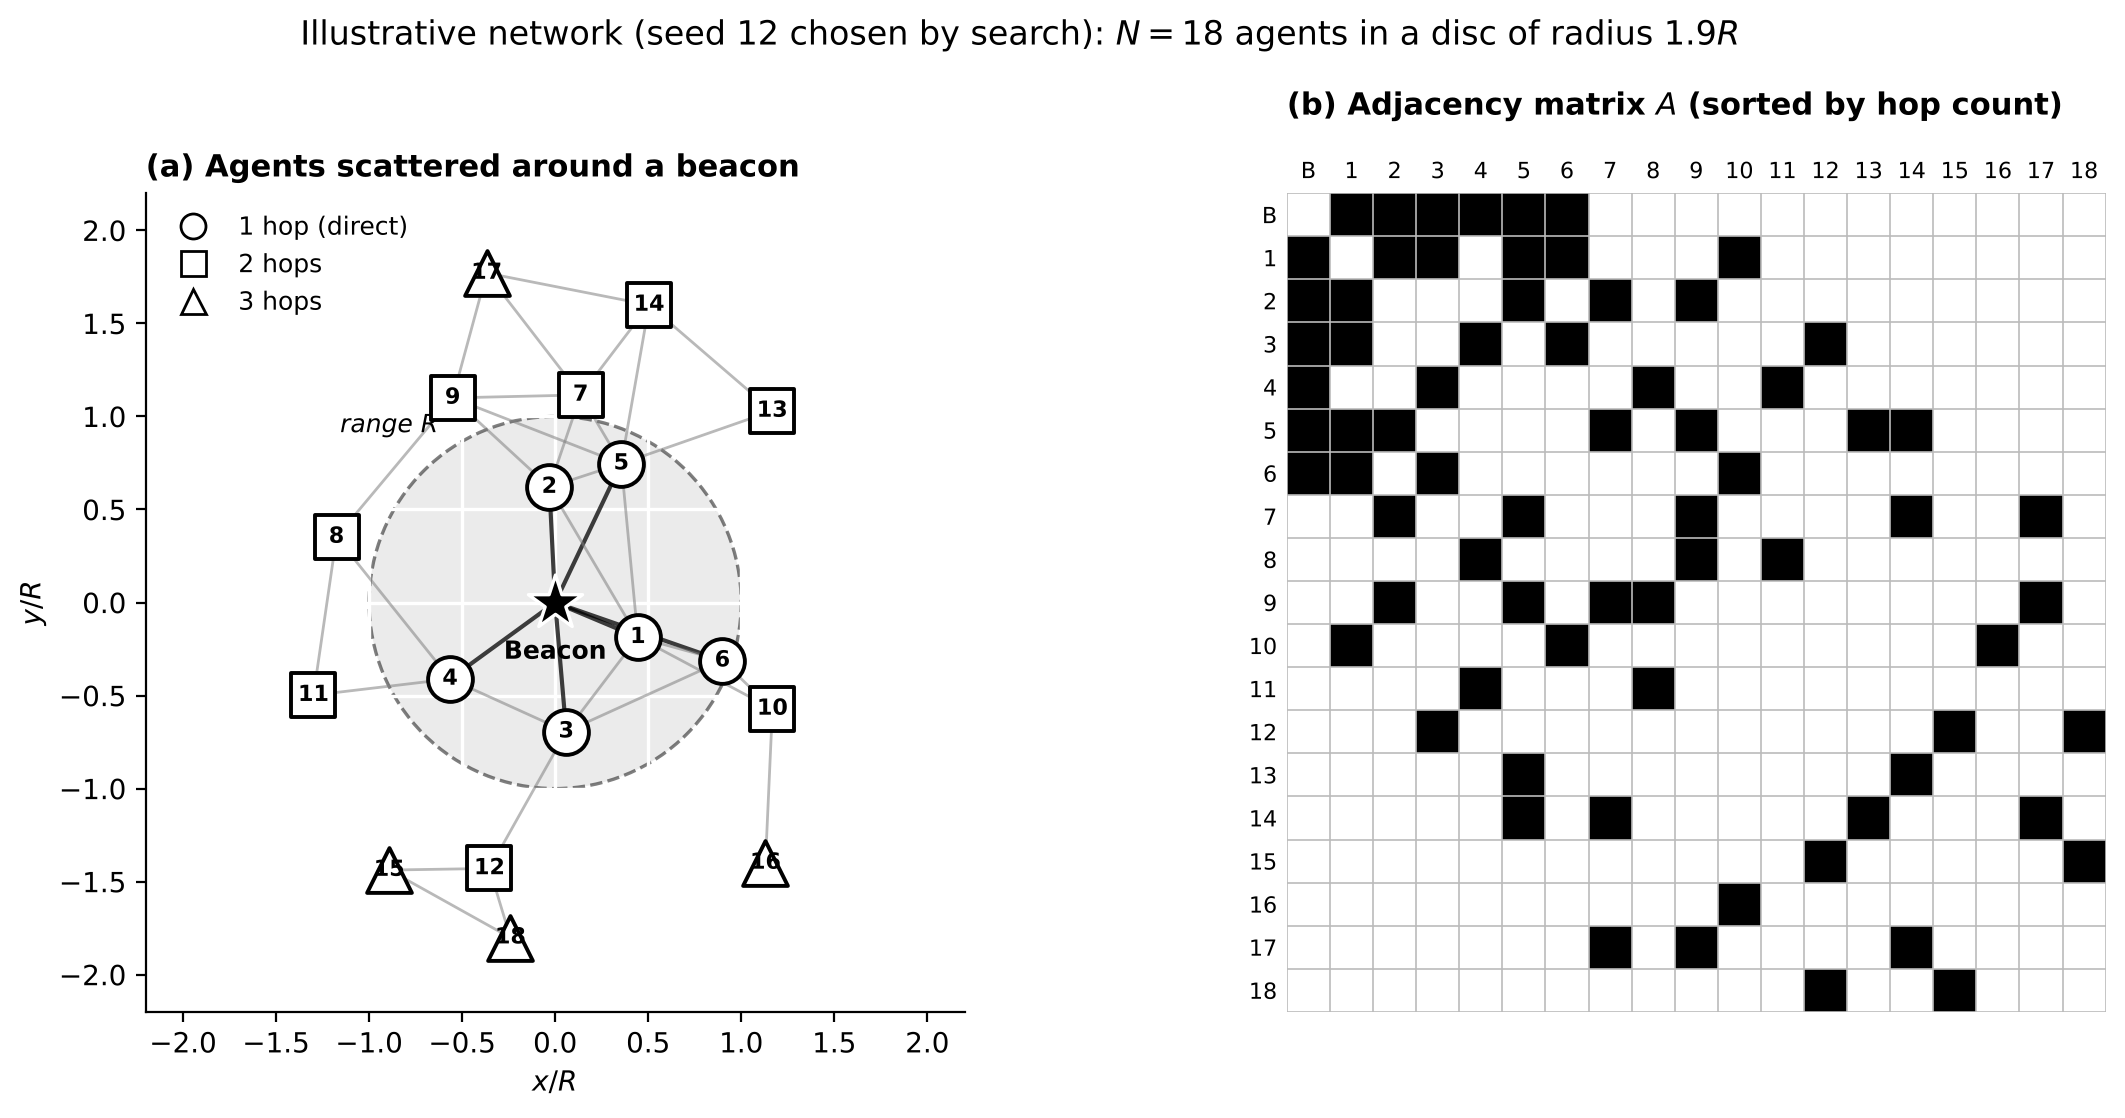
\includegraphics[width=\columnwidth]{figures/fig_connectivity_bw.png}
\caption{Illustrative network, $N=18$, $R=1$ (beacon\,=\,star; circles, squares, triangles\,=\,1, 2, 3 hops). Seed 12 was found by searching seeds for a beacon degree of 6 and a maximum of 3 hops, so this is an \emph{example}, not evidence about how often such networks occur. Redrawn in greyscale from \texttt{beacon\_sim.py}.}
\end{figure}

\textbf{Limits of the model.} (i) Links are treated as on or off and the same both ways; real radio links need not be, which is why C6 is open until measured. (ii) The project has 10 participants, not 18. (iii) Agent-to-agent links and hop counts appear only in the example and figure; they are outside the proposal's scope.



\end{document}
